%%%%%%%%%%%%%%%%%%%%%%%%%%%%%%%%%%%%%%%%%
% University/School Laboratory Report
% LaTeX Template
% Version 3.1 (25/3/14)
%
% This template has been downloaded from:
% http://www.LaTeXTemplates.com
%
% Original author:
% Linux and Unix Users Group at Virginia Tech Wiki 
% (https://vtluug.org/wiki/Example_LaTeX_chem_lab_report)
%
% License:
% CC BY-NC-SA 3.0 (http://creativecommons.org/licenses/by-nc-sa/3.0/)
%
%%%%%%%%%%%%%%%%%%%%%%%%%%%%%%%%%%%%%%%%%

%----------------------------------------------------------------------------------------
%	PACKAGES AND DOCUMENT CONFIGURATIONS
%----------------------------------------------------------------------------------------

\documentclass{article}

\usepackage[version=3]{mhchem} % Package for chemical equation typesetting
\usepackage{siunitx} % Provides the \SI{}{} and \si{} command for typesetting SI units
\usepackage{graphicx} % Required for the inclusion of images
\usepackage{natbib} % Required to change bibliography style to APA
\usepackage{amsmath} % Required for some math elements 
\usepackage{enumerate} % Required for the enumerate function
\usepackage[siunitx]{circuitikz} % Required for the drawing of circuit diagrams
\usepackage{caption}
\usepackage{graphicx}
\usepackage{subcaption}
\usepackage{xfrac}
\usepackage{float}
\usepackage{enumitem}
\usepackage{chemgreek}
\usepackage{pgfplots}
\usepackage{booktabs}

\setlength\parindent{0pt} % Removes all indentation from paragraphs

\renewcommand{\labelenumi}{\alph{enumi}.} % Make numbering in the enumerate environment by letter rather than number (e.g. section 6)

%\usepackage{times} % Uncomment to use the Times New Roman font

\graphicspath{{./fig/}}

%----------------------------------------------------------------------------------------
%	DOCUMENT INFORMATION
%----------------------------------------------------------------------------------------

\title{Analogue Devices \\ Experiment 2 \\ ENG471} % Title

\author{Shane \textsc{Reynolds}} % Author name

\date{\today} % Date for the report

\begin{document}

\maketitle % Insert the title, author and date

\begin{center}
\begin{tabular}{l r}
Date Performed: & April 7, 2016 \\ % Date the experiment was performed
Instructor: & Dr Sina Vafi % Instructor/supervisor
\end{tabular}
\end{center}

% If you wish to include an abstract, uncomment the lines below
% \begin{abstract}
% Abstract text
% \end{abstract}

%----------------------------------------------------------------------------------------
%	SECTION 1
%----------------------------------------------------------------------------------------

\section{Objective}

Explore both the differential and common mode gains of a differential amplifier which is driven by  a current mirror current source.

%----------------------------------------------------------------------------------------
%	SECTION 2
%----------------------------------------------------------------------------------------

\section{Process \& Results}

The differential amplifier implemented in software simulation can be seen in both Figures 1, whis has been set up to find the differential gain, and Figure 2, which was used to find the common mode gain. In both cases, the circuit consists of a current mirror stage and the amplifier itself. A capacitor has been employed to decouple the small signal at the output, $v_0$, from DC sources. To determine the differential gain, the gate of transistor M1 was connected to a sinusoidal voltage source, and the gate for transistor M2 was grounded. This arrangement can be seen in Figure 1. To determine the common mode gain, the gate of transistor M2 was connected to the same sinusoidal voltage source as transistor M1. In both cases a frequency sweep was performed on the sinusoidal input voltage, $v_1$, and the differential voltage gain, $\frac{v_o}{v_1 - v_2}$, or the common mode voltage gain, $\frac{v_o}{v_1 + v_2}$, was measured. These gains were measured for two different loads at the output: 10$\si{\mega\ohm}$ and 400$\si{\kilo\ohm}$. The results for the simulated gain can be seen in Table 1. Hand calculations which support the simulation can be found in calculations section of the report.

\begin{figure}[H]
	\hspace{-3em}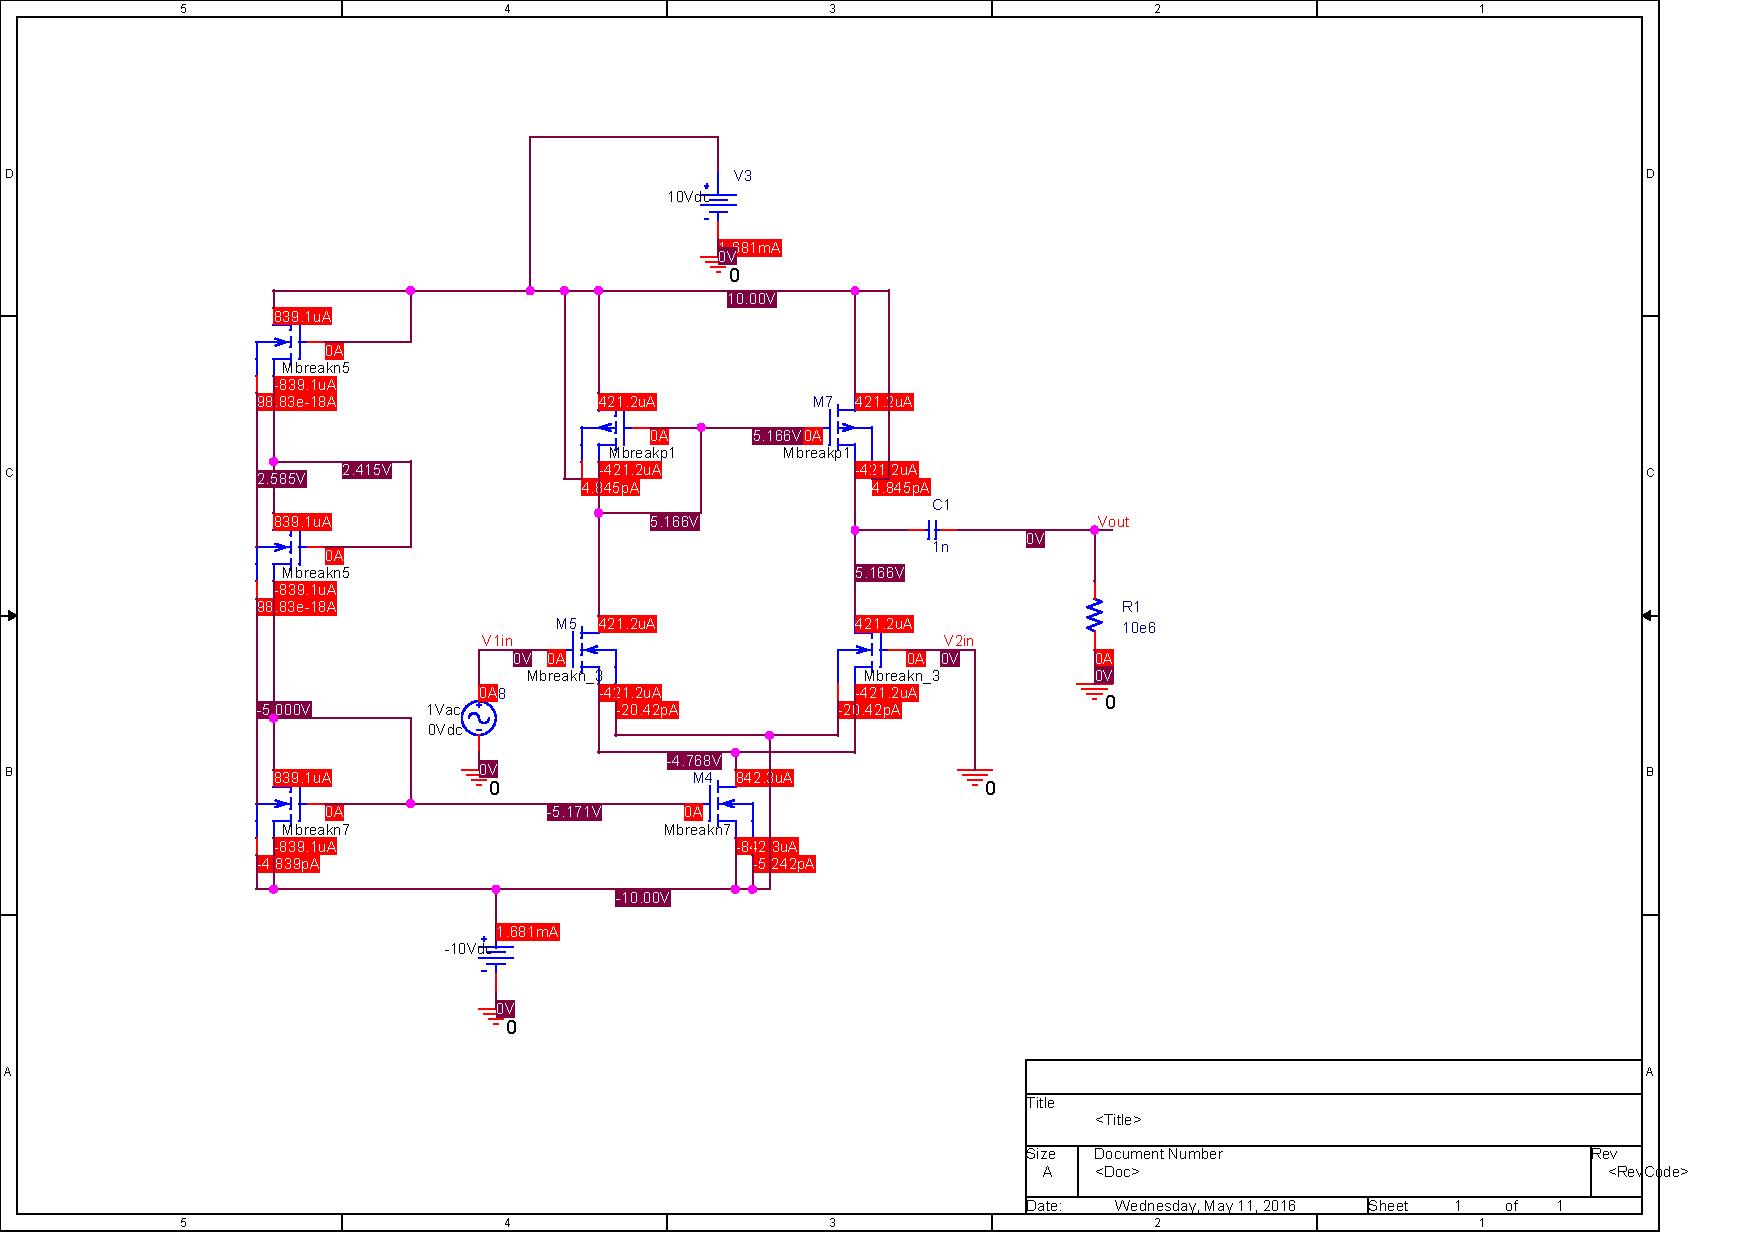
\includegraphics[scale=0.5]{pic1.pdf}
	\captionof{figure}{Simulation for calculating differential gain}
\end{figure}

%----------------------------------------------------------------------------------------
%	SECTION 3
%----------------------------------------------------------------------------------------

\section{Discussion}

The hand calculations for the differential gain came to approximately 35.76 $\sfrac{V}{V}$ for the 10$\si{\mega\ohm}$ resistive load, and 27.07$\sfrac{V}{V}$ for the 400$\si{\kilo\ohm}$ resistive load. Further, the common mode gain for the 10$\si{\mega\ohm}$ load was -0.0134$\sfrac{V}{V}$, and the 400$\si{\kilo\ohm}$ load has -0.00847$\sfrac{V}{V}$. These results closely match the simulated values for the differential gain and common mode gain. Figures 3 and 4 show the results of a simulated frequency sweep for the differential gain of the 10$\si{\mega\ohm}$ and 400$\si{\kilo\ohm}$ loaded circuits, respectively. Further, 5 and 6 show the common mode gain for the 10$\si{\mega\ohm}$ and 400$\si{\kilo\ohm}$ loaded circuits, respectively.\\

\begin{table}[H]
	\centering
	\captionof{table}{Data for differential and common mode gain captured from simulations}
	\begin{tabular}{S[table-format=3.2] S[table-format=3.2] S[table-format=3.2]}
		\toprule
		{Load Value} 	& {$A_d$} & {$A_{cm}$}\\
		{($\si{\ohm}$)}	& {($\sfrac{\si{\volt}}{\si{\volt}}$)} & {($\sfrac{\si{\volt}}{\si{\volt}}$)}\\
		\midrule
		{$10 \times 10^6$}	&	38.01	&	{$12.8 \times 10^{-3}$}\\
		{$400 \times 10^3$}	&	29.16	&	{$9.8 \times 10^{-3}$}\\
		\bottomrule
	\end{tabular}
\end{table}

The DC bias values for which the amplifier's bias currents are derived are shown on the OrCAD schematics in Figure 1. These match the hand calculated results almost identically indicating that the simulation provides accurate results. In fact, error in the simulation is not discernible, however, further understanding of divergence between the hand calculated model and simulated model would require a working knowledge of the computational simulation methods employed by OrCAD. It must also be noted that the hand calculation relies on simplification of the non-linear transistor model and hence contains error of its own.\\

\begin{figure}[H]
	\hspace{-3em}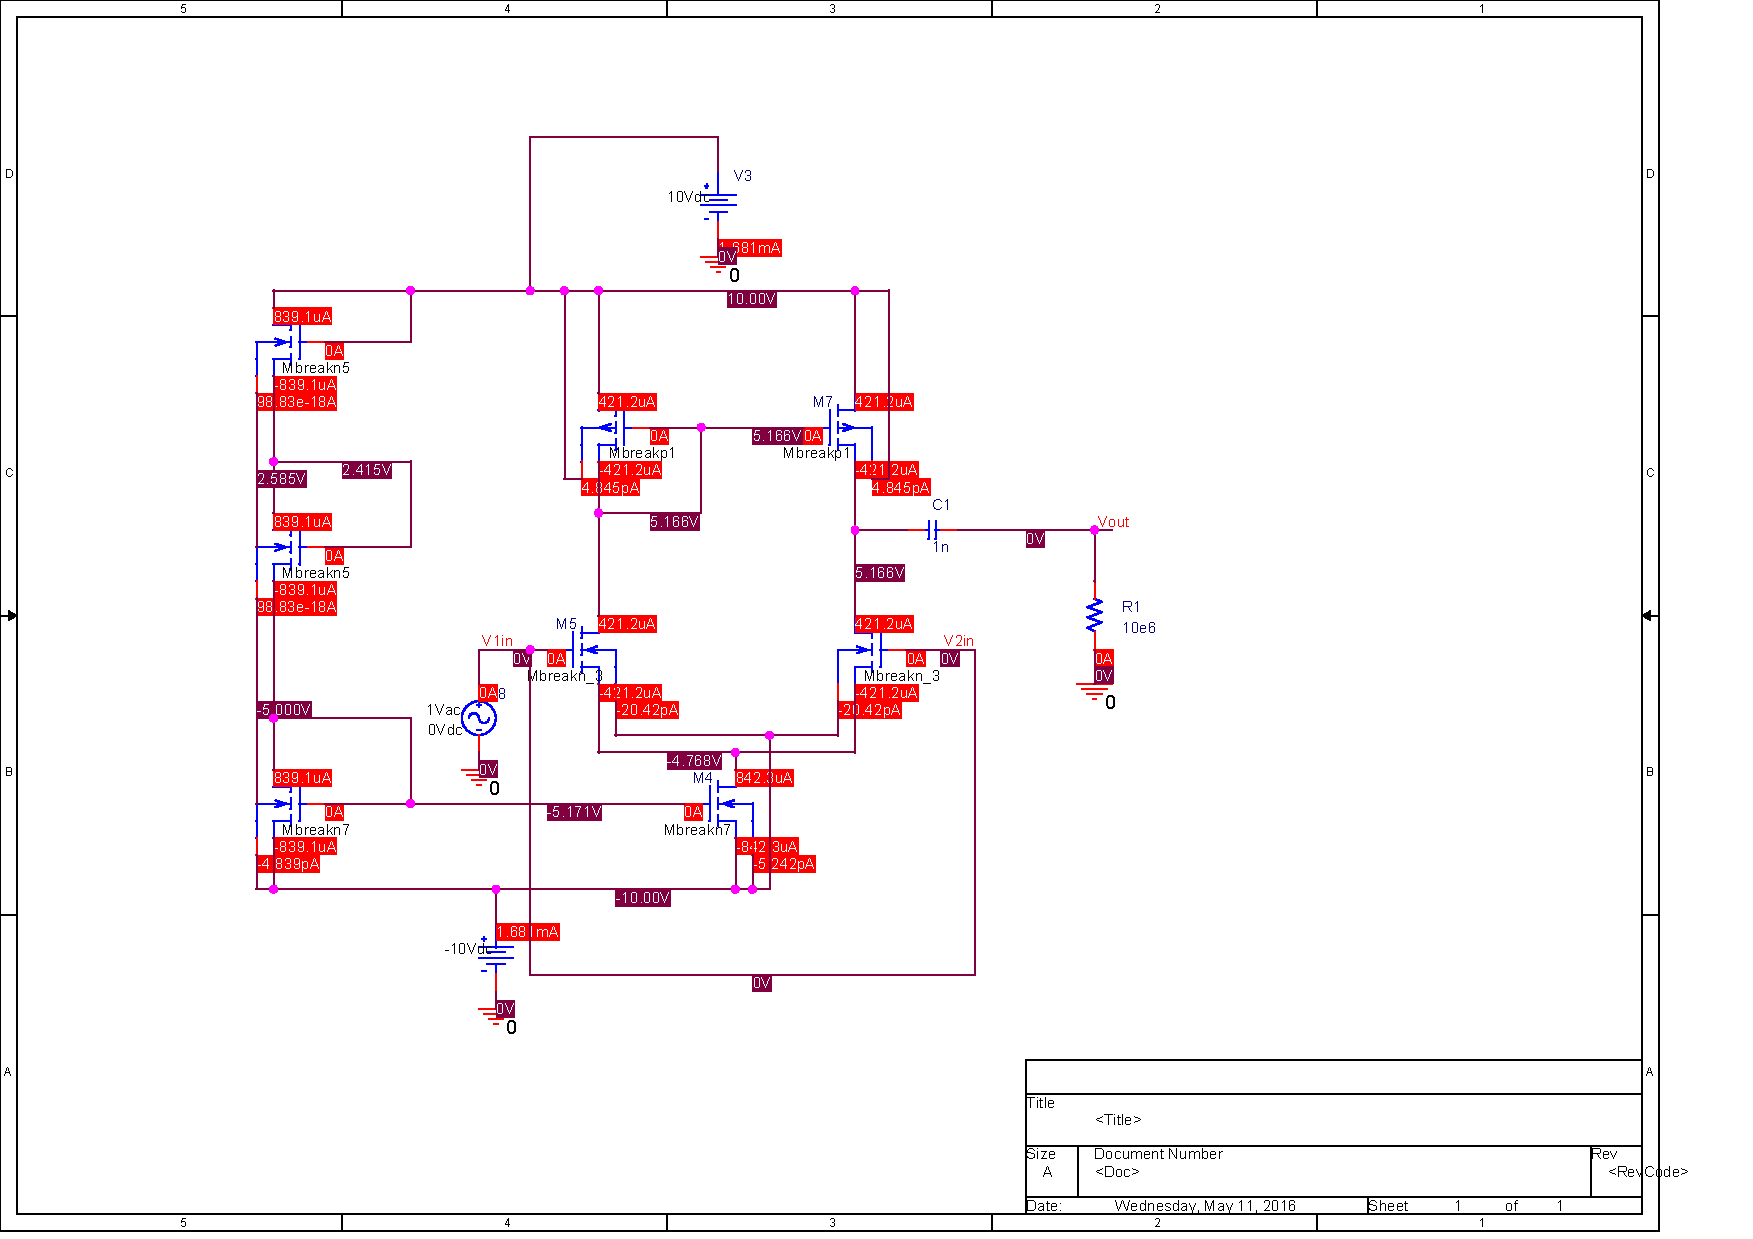
\includegraphics[scale=0.5]{pic2.pdf}
	\captionof{figure}{Simulation for calculating common mode gain}
\end{figure}

\newpage

\begin{figure}[H]
	
	\begin{minipage}{0.5\textwidth}
		\centering
		\begin{tikzpicture}[scale=0.6]
		\begin{axis}[
		xmode=log,
		xmin=10, xmax=10000000000,
		ymin=0, ymax=45,
		scale only axis,
		xlabel=Frequency (Hz),
		ylabel={Voltage Gain [$\sfrac{V}{V}$]}
		]
		\addplot [no markers] table [x=X, y=Y, col sep=comma]{./data/data1.csv};
		\end{axis}
		\end{tikzpicture}
		\caption{Differential gain:\\ $R_L = 10 \si{\mega\ohm}$}
	\end{minipage}
	\begin{minipage}{0.5\textwidth}
		\begin{tikzpicture}[scale=0.6]
		\begin{axis}[
		xmode=log,
		xmin=10, xmax=10000000000,
		ymin=0, ymax=32,
		scale only axis,
		xlabel=Frequency (Hz),
		ylabel={Voltage Gain [$\sfrac{V}{V}$]}
		]
		\addplot [no markers] table [x=X, y=Y, col sep=comma]{./data/data3.csv};
		\end{axis}
		\end{tikzpicture}
		\caption{Differential gain:\\ $R_L = 400 \si{\kilo\ohm}$}
	\end{minipage}
	
\end{figure}




\begin{figure}[H]
	
	\begin{minipage}{0.5\textwidth}
		\centering
		\begin{tikzpicture}[scale=0.6]
		\begin{axis}[
		xmode=log,
		xmin=10, xmax=10000000000,
		ymin=0, ymax=0.015,
		scale only axis,
		xlabel=Frequency (Hz),
		ylabel={Voltage Gain [$\sfrac{V}{V}$]}
		]
		\addplot [no markers] table [x=X, y=Y, col sep=comma]{./data/data2.csv};
		\end{axis}
		\end{tikzpicture}
		\caption{Common mode:\\ $R_L = 10 \si{\mega\ohm}$}
	\end{minipage}
	\begin{minipage}{0.5\textwidth}
		\centering
		\begin{tikzpicture}[scale=0.6]
		\begin{axis}[
		xmode=log,
		xmin=10, xmax=10000000000,
		ymin=0, ymax=0.012,
		scale only axis,
		xlabel=Frequency (Hz),
		ylabel={Voltage Gain [$\sfrac{V}{V}$]}
		]
		\addplot [no markers] table [x=X, y=Y, col sep=comma]{./data/data4.csv};
		\end{axis}
		\end{tikzpicture}
		\caption{Common mode:\\ $R_L = 400 \si{\kilo\ohm}$}
	\end{minipage}
	
	
	
\end{figure}

\begin{figure}[H]
	
\end{figure}

%----------------------------------------------------------------------------------------
%	SECTION 3
%----------------------------------------------------------------------------------------

\section{Conclusion}

The active loaded differential amplifier was analysed using both hand analysis and a computational approach using software to find the differential and common mode gains. Calculated and simulated results differ only marginally. This difference can be attributed to the approximations that are made in the hand calculations. The principal point of difference is that the software did not report an inverted small signal upon amplification.

\end{document}